\documentclass[12pt]{report}
\usepackage[utf8]{inputenc}
\usepackage[english]{babel} 
\usepackage[T1]{fontenc}
\usepackage{parskip}
\usepackage{setspace}
\usepackage[margin=3cm]{geometry}
\usepackage[
backend=biber 
]{biblatex}
\usepackage{csquotes}
\usepackage{fancyhdr}
\usepackage[colorlinks = true,
            linkcolor = black,
            urlcolor  = black,
            citecolor = black,
            anchorcolor = blue]{hyperref}
\usepackage{array}
\usepackage{titlesec}
\usepackage{graphicx}
\usepackage{booktabs}
\usepackage{array}
\usepackage{amsmath}

\addbibresource{literature.bib}

\pagestyle{fancy}  
\fancyhf{}
\renewcommand{\chaptermark}[1]{\markboth{#1}{}}
\lhead{\leftmark}
\cfoot{\thepage}

\fancypagestyle{plain}{
\fancyhf{}
\renewcommand{\headrulewidth}{0pt}
\cfoot{\thepage}
}

\titleformat{\chapter}[hang]{\normalfont\huge\bfseries}{\thechapter}{20pt}{\Huge}
\titlespacing*{\chapter}{0pt}{0pt}{40pt}


\begin{document}

\begin{titlepage}

	\sffamily
    \large
	\begin{flushleft}
	   \doublespacing
	    Leipzig University 				   \\
	    Faculty of Mathematics and Computer Science \\
	    Institute of Computer Science				   \\
	\end{flushleft}
	
	\begin{center}
        \vspace{4cm}	
		\large
		Seminar Paper \\
		
		\Huge
		Problem Solving Tools \\
        \textbf{Measurement Problems}\\
      
        
        \vspace{5mm}
        
        \large
		in the module \\
        Seminarmodul Angewandte Informatik
	\end{center}
	
	\vfill

    \renewcommand{\arraystretch}{1.5}
	\begin{tabular}{ll}
	        Supervisor:     & Prof. Dr. Hans-Gert Gräbe \\
			Submitted by: 	& Victor Jüttner \\
			Email Adresse: & \multicolumn{1}{p{7cm}}{ 
			\href{mailto:vj54cuxa@studserv.uni-leipzig.de}{vj54cuxa@studserv.uni-leipzig.de}
			} \\
			& \\
			Leipzig, \today
	\end{tabular}
	
\end{titlepage} 


\pagenumbering{Roman}
\thispagestyle{plain}
\tableofcontents
\clearpage

\newpage
\pagenumbering{arabic}
\onehalfspacing

\chapter{Measurement Problems}

In our everyday world, measuring mostly doesn't pose any difficulties.
Let's take baking a cake as an easy example.
If you want to bake a cake, you'll have a recipe with all required ingredients in the correct amounts.
A good kitchen has all the tools needed to measure the amounts: a measuring cup for the milk, a scale for the flour or simply your mind to count the eggs.
In this example, it is very intuitively what must be measured.
The given amounts of ingredients are essential. 
Too little or too much could ruin the cake.
Of course all ingredients are needed to get the cake right, none can be left out.
It's also clear what measurement tool is needed for which ingredient.
One would be very lost if they were to measure the circumference of the eggs or weigh ingredients that don't go in the cake at all.
Because this is a simple example, we easily realize that unnecessary measurements are absurd.

Measuring turns more into a problem when we are confronted with more abstract cases.
An example of this is the measuring of code quality.
Now the tools required to measure aren't as obvious anymore, it's also not as easy to know what exactly to measure.
One of the first questions that come to mind is why even measure code quality?
Measuring code quality is needed to verify its readability, maintainability and reusability.
To control these three aspects, we have a variety of variables we can measure: the complexity of the code, the number of defects in the code or whether standards have been followed or not.
Lastly, we need to know how we can measure those variables. 
We can count the comment lines, lines of code or calculate defect density.
These are only very few options of why, what and how to measure code quality.
In this more abstract example, where things aren't as clear anymore, it's much easier to commit unnecessary or even wrong measures.
This is why we need methods to prevent "measuring the circumference of the eggs".

In the context of business are also countless variables that can be measured: financial success, customer satisfaction, production cost, brand value, product quality.
To only name a few.
Here we face the same diffuclties about why, what and how to measure as in the example the the code.
Darrell Mann introduces a variety of tools to overcome problems with measuring in the business world \cite{darrell2004hands}.
In the following pages we'll analyze Mann's tools and discuss the methods for solving measurement problems.

















\chapter{Strategies For Handling Measurement Problems}

\section{What can we measure and why should we?}

Managers love measurements to explore the business world.
There is a vast amount of literature on this topic that comes with idiomatic expressions to help remember principles:

\begin{itemize}
	\item You don't fatten a cow by weighing it.
	\item What gets measured gets done.
	\item The most important numbers are unknown and unknowable.
\end{itemize}

Those expressions contain guidelines for core questions for good measurement.
The first expression deals with the correct amount of measuring, the second with the correct form and the third with intangible factors.
Since expressions are rather vague, we will introduce the ideality equation in \autoref{ideq}, which is used in the entire systematic innovation methodology.
With the equation we have a powerful tool to better understand connections and problems in the business world 

\begin{figure}[h]
	\centering
	\begin{equation*}
		\text{Ideality} = \text{Perceived} \left(\frac{\text{Benefits}}{\text{Cost} + \text{Harm}}\right)
	\end{equation*}
	\caption{Ideality equation as used by Darrell Mann }
	\label{ideq}
\end{figure}

Wherever the equation is applied, only the variables \textit{perceived}, \textit{benefits}, \textit{cost} and \textit{harm} justify measuring in the context of business.
With this the ideality equation helps us with the question of what to measure, so it's worthwhile to take a closer look to its components.
\textit{Cost} is just the monetary cost and therefore easy to measure, due to this it receives the most attention.
To understand \textit{benefits} it's best to take the viewpoint of the receiver, the customer.
Benefits depend on how much value the customer sees in the product or service offered.
\textit{Harm} is intended to show wastefulness and how sustainable and environmentaly friendly the system is.
"The most important numbers are unknown and unknowable", the third of the expressions to help understand measurements hints to the variable \textit{perceived}.
The three first variables \textit{benefits}, \textit{cost} and \textit{harm} are rather straightforward and can be measured with fiscal means.
Sadly \textit{ideality} can't be measured this easily.
We also need to consider the amount of uncertainty and complexity that exist due to the intangible factors.
\textit{Perceived} is meant to measure those intangible factors.

We now know that these four are the variables that need to be measured.
But let's take a step back and have a look at a system to understand why measuring is even needed.

\begin{figure}[h]
	\centering
	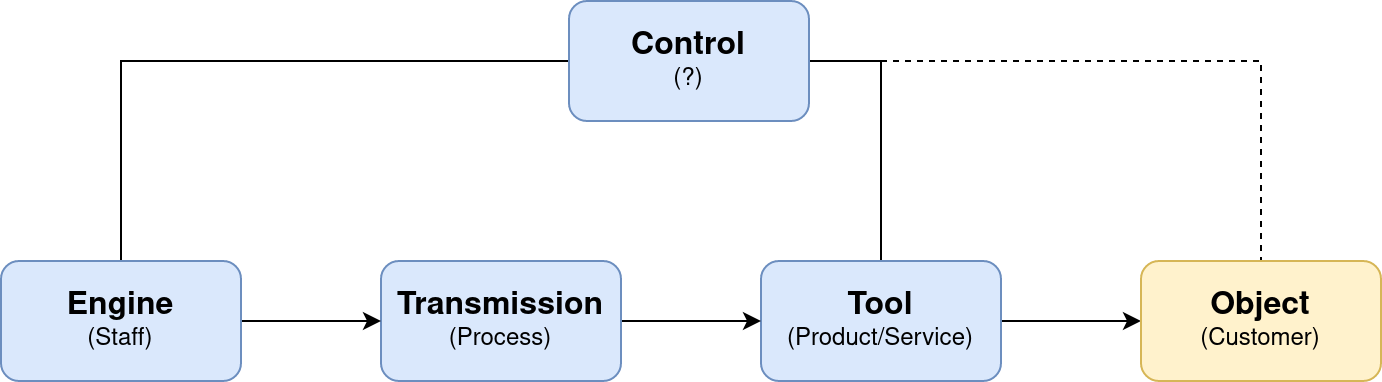
\includegraphics[width=\textwidth]{control3.png}
	\caption{Feedback and Control in a viable System (adapted from D. Mann "Hands on Systematic Innovation for Business and Management", p. 354)}
	\label{viable}
\end{figure}

In \autoref{viable} we see the essential elements in a viable system.
The productive system consists of staff that produces products or services via a process.
At the end of this process there is an object that the customer receives.
Above this productive system is the control instance.
Control is the part that deals with measurement data and control information.
Without control and the measurement that is needed for it, the productive system wouldn't be viable.
To measure viability, the ideality equation is used.
It is sufficient to measure the overall ideality of a system instead of the individual variables of the formula.

The viable system shows us why it is important to measure, a system wouldn't work without it.
Another, more practical approach to the question of what and why to measure is given by the APQC.
"Create and manage [a] organizational performance strategy", this strategy by the APQC contains measuring, tracking, streamlining and improving internal performance.
For this paper, we only care for the five measurement processes: enterprise measurement system, process productivity, cost-effectiveness, staff efficiency, and cycle time \cite{apqc}.
According to the APQC this process should be measured to efficiently evaluate a business process.

Darrell Mann points out one more important point that concerns measuring: complexity.
Systems follow an evolution trend of increasing and decreasing complexity.
Complexity is introduced and increases steadily in a system due to the need for measurements.
Without the data obtained with measurements, it is very difficult to understand or improve a system.
For this reason more and more methods for taking measurements get introduced into a system.
Those methods increase complexity up to a point of maximum viable complexity.
When the point of maximum viable complexity is reached, cost and reliability start to decline.
Therefore, the complexity must be reduced, which can happen by removing methods of measurements.

\begin{figure}[h]
	\centering
	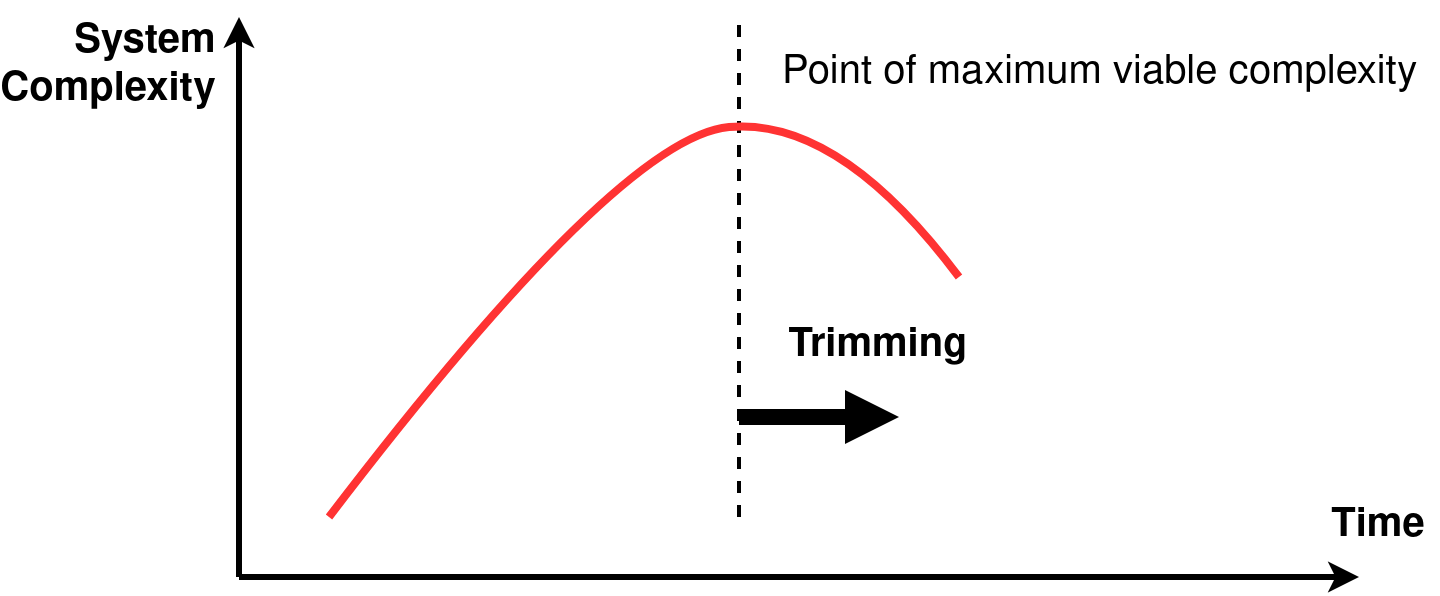
\includegraphics[width=\textwidth]{complexity2.png}
	\caption{Complexity Trend (adapted from D. Mann "Hands on Systematic Innovation for Business and Management", p. 355)}
\end{figure}

Measurements are necessary in a system to understand it; when this has happened the measurements should be removed or integrated to reduce the complexity.
This trend of rising and falling complexity helps us understand when it is needed to install measurements and when to remove or integrate them.


\section{How to measure}

To find a solution on how to measure, Darrell Mann has compiled a list of strategies.
This is a best practice list for measurement from several hundreds of thousands of interdisciplinary examples.
Mann's list follows a top-down approach, so that solutions from the top of the list are more ideal than the following.
Therefore, it is better to implement one of the higher-up strategies than to look further down the list.
The strategies are generic, but each one has added content and examples to better understand them.

List contains many elements of class 4 "measurement and detection in substance-field systems" of the 76 standards.
However, Mann doesn't introduce the substance-field system for his list, which class 4 is based on.
Compared to the 76 standards, Darrell Manns methods are more practical solutions; they are a "hands-on approaches" for the business context instead of a general guideline for measurement.
Furthermore, many of the methods from the 76 standards are in a different order than Mann's list.
Where possible we want to enrich Manns list with additions from class 4 of the 76 standards \cite{koltze}.


\subsection[Eliminate the need for measurement]{Modify the system so that there is no need to make the detection or measurement}

Since measurements can increase the complexity of a system, it makes sense that we should try to avoid them.
Therefore, the first strategy is to modify the system so that the detection or measurement is not needed.
There are several ways to eliminate the need for measurement or extra measurements.
Remember the idiomatic expression "you don't fatten a cow weighing it", suggesting not to take unnecessary measurements.
If the information provided by a measurement has no useful function, it should just be eliminated.
Another approach is to make measurements out of already existing data.
Instead of introducing a new means for measuring it should be tried to make the measurement on existing data.
An example: motion-sensitive lighting can not only be used to safe energy but also to show when people are in the office.
It can be difficult to know what measurements and data already exist.
Transparency inside of an organization can eliminate this problem.
Not only can a broader overview of all the data be used to further integrate measurements but transparency also allows to eliminate measurements completely, that are only there to understand workings in the company itself.
The last approach to this strategy is to integrate measures into one another, so that one measure can provide information for one or more functions.


\subsection[Measure on copy]{Make the detection or measurement on a copy, image or replica of the object or system}

If it is not possible to eliminate the measurement or detection, it is recommended to use a copy, image or replica of the system for the measurement.
For example, it could be dangerous to measure the length of a venomous snake.
It is much safer to make a picture of the snake and measure its length via proportions.
Other great tools to create a copy can be simulation or scenario planning software.
To gain real world information out of their own user base, many companies implement beta test networks.
The beta test network provides a microcosm in which experiments can be conducted and measurements taken without interrupting the regular user base.
The film industry uses test audiences to achieve something similar.
A test audience is supposed to be a representative sample of the full market.
If separate groups can not be implemented customer feedback measurements can also be gained via internet-based forms.


\subsection[Measure changes]{Transform the problem into one involving successive measurement of changes}

This strategy is to measure the change in a system.
It is especially suited for systems with recurrent and sequential measurements.
The differences or deltas between the measurements can be used to gain additional knowledge.
In a computer program, short distances in time between key-presses or mouse-clicks can indicate proficiency in this program or can reveal that a user is new.
An automobile on the other hand, could use the slower than normal reaction time of its user as an indicator for driving under the influence.
Measurements of differences can also provide further information for the measurements themselves.
If there is little to no change between measures, the frequency of measurements can probably be reduced.
Very drastic changes in measured values could indicate to measure more often.
A high rate of measure frequency changes could also indicate non-linearities or abnormalities.

\subsection[Add new element to measure]{Add a new element (communication or person or element) to provide an easily detectable parameter related to the parameter required to be measured or detected}

This is the first strategy that introduces a completely new entity into a system in order to make a measurement.
The idea is to provide an easily detectable parameter that is close and similar to the parameter that is going to be measured or detected.
To measure the quality of customer service mystery shoppers are often used.
These are people that have an invented problem with which they have to navigate customer service.
With the information they provide, the quality and speed of the service can be rated.
Another popular method are suggestion schemes.
They are a tool to generate ideas and can be an indicator for an organizations morale and health.
But feedback doesn't even need to be as complicated as a scheme.
With the introduction of a physical or virtual notice-board people can easily contribute data and information.
More technical approaches include cookies to collect information on how a user navigates and uses a website or GPS tracking systems to easily locate persons or goods.


\subsection[Add detectable element]{If it is not possible to modify the system, then introduce an easily detected element to the surrounding environment}

If a system can not be modified by a new element to make the measurement or detection, the new element can be introduced in the systems surroundings.
It still is important that the added element is easily detectable.
Such elements could be CCTV cameras to observe the perimeter of the system or an external temporary consultant, who is hired to make the measurements.
Even though this strategy is just concerned with the surroundings of a system and not the system itself, it is important to keep heisenbergs uncertainty principle in mind.
Any attempt, even though it does not directly modify the system, will change the system.


\subsection[Measure changes within system surroundings]{If it is not possible to introduce an easily detectable element into the environment surrounding a system, obtain the desired measurement by detecting changes in something already in the environment}

The sixth strategy again utilizes changes in between measurements.
It should only be used if no new element can be introduced in a system or its surroundings.
The idea is to obtain measurements from changes in the environment surrounding the system.
To gain information on morale, it can be useful to interview friends and family of the organizations staff.
Also, it can be worthwhile to follow the press closely, since they are usually sensitive to changes in the world which can help to sense disruptions.
If the system deals with crowds of people, noise levels can be an indirect indicator of enjoyment.
High background noise can indicate low enjoyment, but high noise due to clapping or cheering could also indicate high enjoyment.


\subsection[Psychological effects]{Make use of psychological effects to help make the measurement}

With this strategy we leave the direct measurements and introduce strategies to help make measurements.
Darrell Mann introduces some psychological effects that one should keep in mind when working with people.
These points can help to convince people to commit to other strategies.
For example, even though it feels contradictory, telling someone they can not have something is a good way of making them want it.
Another contradictory action is to not tell people too much.
The more you tell people, the more they could think you're hiding.
Most people want to feel included; this is why you should use inclusive language when formulating questions.
People also need a certain amount of stimulus before they commit, it can help to have elements that activate stimulus.
Last but not least, keep in mind that bad news travels faster than good news.


\subsection[Emotional effects]{Use emotional effects to help to make the measurement}

The strategy for working with emotional effects is the same as the one for psychological effects; it is an aid to make measurements by influencing people on an emotional level.
For this strategy it is essential to know ones user base so that the exciters and "hot buttons" of customers can be identified.
Emphatic listening can be another mean to build a connection to a person in order to motivate them to commit to measurement strategies or reveal their real thoughts. 


\subsection[Measure the opposite]{Use the inverse or opposite system to make the measurement}

The last strategy focuses on the opposite of the system that is supposed to be measured.
By measuring things that are not present, space that is not used, or non-customers, information about yet unused elements could be revealed.




\chapter{Case Studies}

Darrell Mann takes a closer look at case studies to analyze measurement problems in the real world.
In this essay we only want to discuss two of those case studies.
One regarding the photographic paper industry, to deepen our understanding of what to measure.
The other regarding project management in general with a closer look on how to measure resources.

\section{Measuring Business Performance}

The digilization has led to the use of less photo-paper.
Digital cameras can delete bad photos instead of printing them; pictures get stored on hard drives, and the film industry has become digital.
Due to this, the photo-paper industry is in front of a conflict.
Less paper will be needed in the future, and the decline of the industry is certain.

Now it is interesting what the industry normally measures to maintain control.
Mostly variables that are easy to measure: sold amount of paper, revenue, costs.
In the day to day business, these measurements are very helpful in adjusting the input and output of the company.
But for the long run looking only at those information won't help with the declining need for photopaper.
We need to take a step back and consider the companies main useful function.
Photo-paper used to be a mean to be able to see photos and to keep and store them.
The function to be able to see them is now obsolete, but the memory function of pictures remains the same.
People love photo albums but it is hard work to organize them.
The industry must realize that their product is mostly used to store memories and be able to revisit them.
This opens up a whole new palette of options.
An online platform could be introduced to store photos and share them with friends and family.
With this in mind, the dimensions that should be measured change completely.
Aspects like most views, most shares, group size of viewers and number of images get much more important.
These are future oriented measurements, but of course they are much harder to measure.

More than ten years have already passed since the publication of Manns book.
We can use this as an advantage to have a look at today's memory business.
Many companies have joined the memory business with similar ideas as proposed in Darrell Manns book.
Apple creates photo albums for you by using the time and location information of the photos.
Different social media platforms create highlight reels of the last year.
Still-standing photos got upgraded to shorter, more vivid video clips.
Even discounter offer to print calendars, photo albums and other merchandise out of your favorite pictures.
This shows that Mann was right with his suggestion to measure the memory function of products, since this function is very much alive.

\section{Project Management System Measurements}

Project management seems to be inherently flawed.
Of all projects, 85\% end either to late, over-budget or under the required specification, sometimes even as a combination of all three.
Many project managers now use a dashboard, similar to that of a car, to have a broad overview of all data.
However the data is organized, it is vital that the data is relevant, acquireable and accurate.
One of the main problems in project management comes out of data acquisition.
If there is not enough data to understand a system, often more project managers get hired to gain more data.
We have seen that this increases the complexity of a system and should be avoided.
Instead, lets apply the first strategy for how to measure: modify the system so that there is no need to make the detection or measurement.
The ideal data acquisition should happen out of existing resources.
Popular systems to get this data would be digital diary and accounting systems, automated reporting, suggestion schemes, or the amount of phone calls.
These are the first sources that should fill a project managers dashboard.
It is so important not to first introduce more project managers because it can lead to individuals losing their sense of responsibility.
If someone else, here the project manager or a quality department, is there to maintain a timeline or standard, the individual could stop caring for being responsible for that measurement themselves, since there is someoone whose job is exactly that.




















\chapter{Conclusion}

To conclude the why, what and how of measuring in the business context, Darrell Mann ends this chapter with his own experiences.
Measurement methods often only need to be reconsidered when a system is in its evolutionary development or when a new function is added to an existing system.
If these stages are suffering from inadequate feedback and control mechanisms, it is important to reconsider ones strategies.
To create appropriate measurement it is best to define in simple functional terms the required data from the system.
Always keep the main useful function in mind and whether a measurement serves to help control this function. 

\newpage
\thispagestyle{plain}
\pagenumbering{Roman} 
\setcounter{page}{2}
\printbibliography[heading=bibintoc]

\end{document}
